\renewcommand{\chaptername}{}

\chapter{METHOD}

Emotions are highly nuanced since there are many experiences that do not fall neatly within a category. 
The difference between bittersweet and nostalgic, for example, is very different to quantify. The six Ekman emotions 
are joy, sadness, anger, fear, disgust and surprise \cite{transprose}.  For this paper we will focus on 
classifying songs based on the first three emotions (joy/happiness, sadness and anger), mainly because there is not enough sample songs whose main
emotions are the last three (fear, disgust and surprise).

\subsection*{Features Used}

The audio features used for the experiment are the timbre data from the EchoNest dataset.
These features are zero-mean vectors of length 12,  extracted by windowing the spectrogram in constant-width segments. 
Although the segment width varies from song to song, it is typically under a second long and it is determined
so that the timbre and harmony are relatively uniform throughout.  

The song is broken up into a series of non-overlapping windows $\mathcal{S}_i$ for the $i^{th}$ segment. 
The images in Figure 1 are a visual representation of the basis functions $g_j$ that were applied to each segment. 
An audio feature $f$ is extracted from each segment and has the form of a vector of length $12$,
 where each element of the vector is defined as follows: 

\[ f_j (x) = \sum_{p \in \mathcal{S}_i} g_j(p) \bullet x(p) \qquad j \in \{1, 2, ..., 12\}\]

The lyric information was obtained from the musicXmatch database \cite{musicXmatchDataset} 
that provides the songs in a bag of words format. This format consists  of a vector of length 5000 representing 
a stemmed dictionary where the value at each element is the number of times that a particular word
is used in the song. Data is distributed in this form so that it respects artists' 
rights over the ordering of the words while still being able to represent the content. 

\begin{figure}[h!]
  \centering
      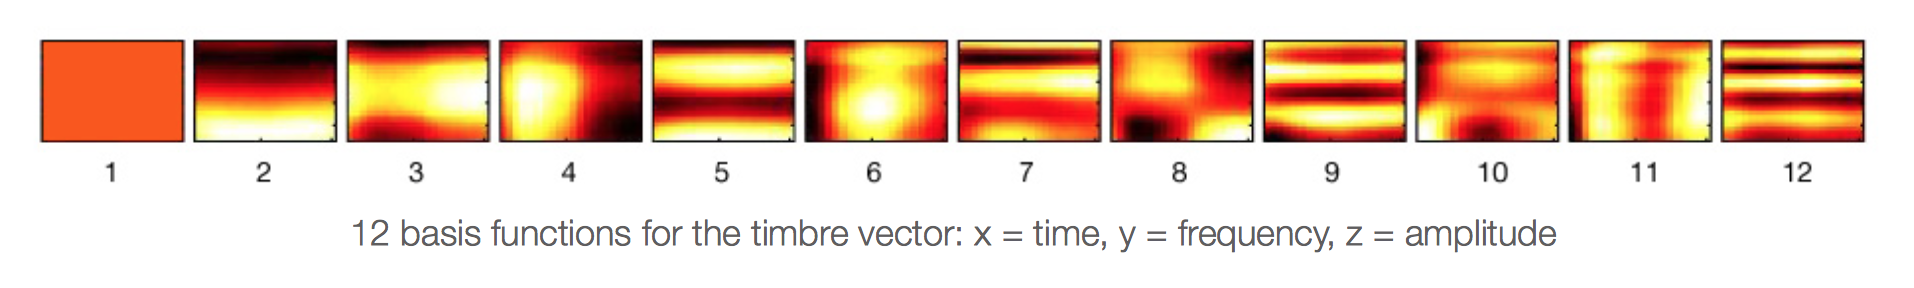
\includegraphics[width=1\textwidth]{BasisFunctions.png}
  \caption[Compact Routing Example]%
    {EchoNest's basis functions used to generate MFCC like vectors.\protect\footnotemark}

  \end{figure}
    \footnotetext{\url{http://developer.echonest.com/docs/v4/_static/AnalyzeDocumentation.pdf}}


\section*{Classifiers}

As mentioned in the Chapter 2, similar problems have been address with
certain amount of success using Naive Bayes and SVMs. For the experiment the 
classifiers selected were the Gaussian Naive Bayes, Multinomial Naive Bayes and 
Kernel SVM with histogram intersection as the kernel. 

\subsection*{Naive Bayes}

The Naive Bayes classifier is a statistical classifier that selects the most-likely 
class given a particular data point. The classifier builds a statistical model for each class that 
follows a given distribution. Under the assumption that each
feature is statistically independent, it computes the conditional probability for 
the input vector given each model and returns the model with the highest probability.

\[ \hat{y} = \text{argmax}_{y} P(y) \Pi_{i=1}^{n} P(x_i|y)\]

The distinction between the Gaussian Naive Bayes and the Multinomial Naive Bayes is the 
distribution that is assumed for the conditional probability $P(x_i | y)$.  The Gaussian Naive
Bayes classifier, as the name suggests, assumes that data is normally distributed and 
that the covariance matrix are diagonal. It is a good 
starting point when little information is known about the data. 

The Multinomial Naive Bayes supposes that data follows a multinomial distribution, which is a generalization 
of the binomial distribution.  The difference between binomial and multinomial is that in binomial the outcome 
of each of the $k$ trials is either "yes" with a probability of $p$ or "no" with a probability of $(1-p)$. Under the multinomial
distribution, the outcome of each of the $k$ trials can be one of $n$ different classes such that $\sum^n_{i=1}p_i = 1$.
Since an event cannot occur a negative number of times, the multinomial distributions is well suited for problems where 
the vectors are non-negative such as for histogram analysis. 

\subsection*{Support Vector Machines}

Support Vector Machines are classifiers that construct hyperplanes that maximize the margin 
to the labeled data points. The margin is defined to be the shortest distance from hyperplane 
to any of the points. As a result a linear SVM finds a function that linearly separates the data
points into clusters for classification. Soft SVMs exist that tolerate data that is not linearly separable by allowing
some misclassification. 

An SVM can be non-linear if the data points are  preprocessed non-linearly before creating the hyperplane. 
Non-Linear SVMs rely on functions called kernels that map data points into a higher dimensional space where
the points can be separated by a single hyperplane. 

For the experiments detailed on this paper, we used a non-linear SVM with a histogram intersection kernel.
Histogram intersection is a method that finds the minimum intersection between two histograms \cite{maji2008classification}, which means 
that it is generally more accurate similarity metric than euclidean distances for histograms.  The histogram intersection kernel is 
defined by the function below:

\[ k_{HI}(h_a,h_b) = \sum_{i = 1}^n min(h_a(i),h_b(i))\]

The formula above details the metric used to compare the intersection of two histograms. The distance of a particular 
pair of histograms is the sum of minimum value of each column of the histogram.  By computing the distance between 
every pair of histograms using this metric, the SVM can easily group similar data points together. 

\begin{figure}
\begin{minipage}[b]{0.6\linewidth}
  \centering
  \hspace*{-.7in}
  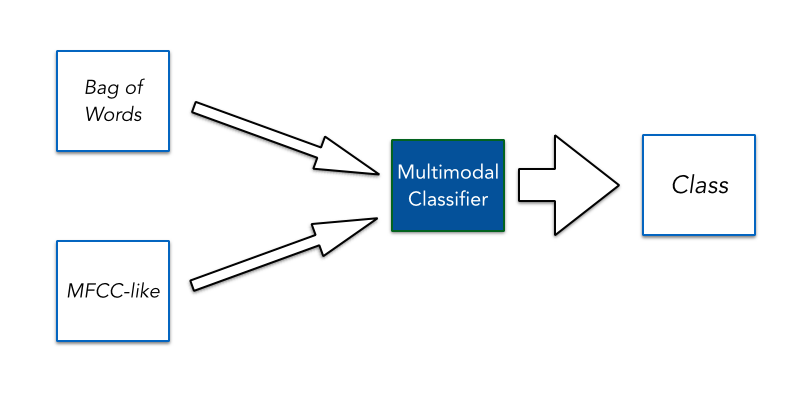
\includegraphics[width=1\textwidth]{Setup001.png}
  \caption{Series Fusion}
  \label{fig:blah1}
\end{minipage}
\hfill
\begin{minipage}[b]{0.6\linewidth}
  \centering
    \hspace*{-.3in}
  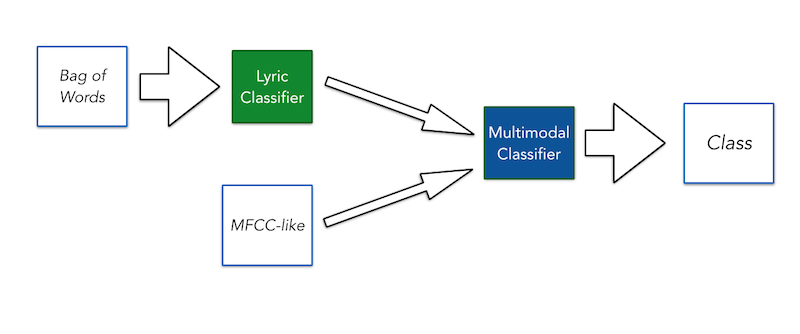
\includegraphics[width=1\textwidth]{Setup004.png}
  \caption{Lyrics Only Partial Ensemble}
  \label{fig:blah2}
\end{minipage}

\vspace{1em} % add some whitespace after the first figure


\begin{minipage}[b]{0.6\linewidth}
  \centering
  \hspace*{-0.7in}
  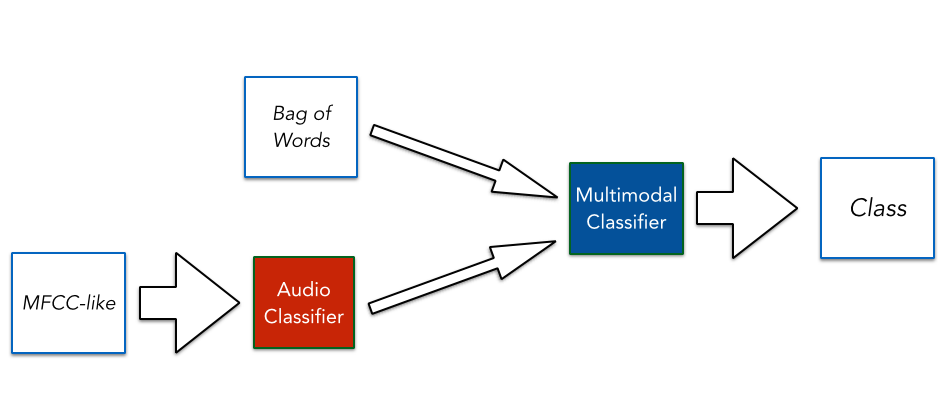
\includegraphics[width=1\textwidth]{Setup002.png}
  \caption{Audio Only Partial Ensemble}
  \label{fig:blah1}
\end{minipage}
\hfill
\begin{minipage}[b]{0.6\linewidth}
  \centering
      \hspace*{-.3in}
  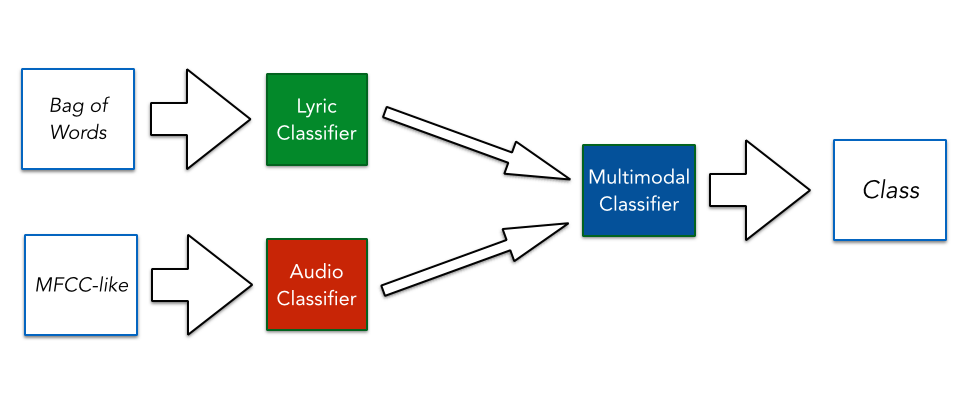
\includegraphics[width=1\textwidth]{Setup003.png}
  \caption{Full Ensemble}
  \label{fig:blah2}
\end{minipage}
\end{figure}


\section*{Fusion Methods}

Using the features and the classifiers detailed above, four different fusion methods were used for 
classification: Series Fusion, two separate Partial Ensemble and Full Ensemble. These were defined by
concatenating the feature vectors at different levels of processing.  The figures above show a graphical 
representation of the different structures implemented.  

It is important to note that out of the classifiers detailed above, only Gaussian Naive Bayes is suited to classify 
negative-valued features. As a result not all the classifiers can be used for all the vectors.   The Multinomial Naive Bayes
classifier requires that audio segments be normalized to be non-negative to be fitted to the multinomial distribution. We introduce the
following classifier sets:

$ \mathcal{A} = \text{set of audio classifiers} = \{ \text{Gaussian NB}, \text{Multinomial NB}\} $

$ \mathcal{L} = \text{set of lyric classifiers} = \{ \text{Gaussian NB}, \text{Multinomial NB}, \text{SVM}\} $

$ \mathcal{M} = \text{set of multimodal classifiers} = \{\text{Gaussian NB}, \text{Multinomial NB}, \text{SVM}\} $


The set $\mathcal{A} $ is used for audio features, the set $\mathcal{L}$ is used 
for lyric features and the set $\mathcal{M}$ is used for multimodal features.  In the figures above, the squares labeled as
Multimodal Classifier, Audio Classifier and Lyric Classifier represent a sampled classifier from the corresponding set.

\subsection*{Series Fusion}

The Series fusion method is the basic approach discussed in the Chapter 2 of this document. This
method concatenates each raw audio vector with the corresponding raw lyric vector. As a result each song has hundreds of segments,
each of which is a vector of length 5012.  This large dataset can be computationally prohibitive for certain classifiers. 
 The classifier set for this structure is : 

\[ \text{Series} = \mathcal{M} \setminus \{ SVM\} \]

The reason why SVMs were not included in this test was because 
the runtime complexity of training an linear SVM is at worst $O(d^2n)$ where $d$ is the number of dimensions and $n$ is the number of samples \cite{chapelle2007training}. 
With a hundred vectors per song where each vector has 5012 dimensions, it becomes impractical to run this test.

This fusion method involves taking a classifier from the set $Series$ and training it on the dataset resulting from the concatenation 
of the audio vectors and bag of words.  

\subsection*{Audio Partial Ensemble}

The Audio Partial Ensemble methods come from noting that the complexity of the Series Fusion method stemmed from the 
fact that the amount of vectors for each of the modes was lopsided. Each song has exactly one bag of words vector of length 5000, while 
having hundreds of audio segments of length 12. Audio Partial Ensemble explores preprocessing those hundreds of segments and representing them as a single
vector that can be combined with the bag of words. 

This method initially classifies all the song's audio segments, and builds a histogram
for each song containing how many of these segments were classified for each emotion. 
As a result the audio data goes from being represented by hundreds of
vectors of length 12, to a single histogram of length 3 that provides some concrete information of the emotional content of the song. 

The classifier set for Audio Partial Ensemble is defined as all the combinations between the Multimodal classifier set and the Audio classifier set.  The resulting 
set is as follows: 

\[ \text{Audio Partial Ensemble} = \mathcal{A} \times \mathcal{M}   \]

For this fusion method a classifier is taken from $\mathcal{A}$, and is used to build the emotional histogram from the audio segments. This 
histogram is then concatenated to the bag of words to create the multimodal vector, which is used to train the classifier from $\mathcal{M}$.


\subsection*{Lyric Partial Ensemble}

The Lyric Partial Ensemble is very similar to the Audio Partial Ensemble, with the modification that the preprocessing is  
performed to the bag of words vector instead of the audio. 

The classifier set for Lyric Partial Ensemble is defined as all the combinations between the Multimodal classifier set and the Lyric classifier set. 

\[ \text{Lyric Partial Ensemble} = \mathcal{L} \times \mathcal{M}   \]


This fusion method takes a classifier from $\mathcal{L}$ and determines the likelihood that each bag of words belong to each class, resulting
in a vector of length 3. This likelihood vector is concatenated to the MFCC-like vectors from the audio data to create the multimodal features. 
A classifier from $\mathcal{M}$ is used to make the final decision based on this vector. 

\subsection*{Full Ensemble}

Taking both Partial Ensembles to the next logical step, Full Ensemble preprocesses both the audio and the lyric vectors and concatenates the 
the intermediate results into a single multimodal vector. The audio vectors are converted into the same emotional histogram used in the Audio Partial
Ensemble method. The bag of words, like in Lyric Partial Ensemble, is used to create a likelihood vector. The emotional histogram and the bag of words classification are concatenated
and used as a single vector for multimodal classification.

The classifier set for Full Ensemble is defined by all combinations between the Audio, Lyric and Multimodal classifier sets. The resulting set is 
defined as follows:

\[ \text{Full} = \mathcal{A} \times  \mathcal{L} \times  \mathcal{M}\]


\chapter{EXPERIMENT}

Given the size of the dataset, it was necessary to perform significant preprocessing for each test to run in a sensible amount of time. The experiments require that every song has audio vectors, a lyric vector and a true emotional label. To get the subset of the Million Song Dataset that had these characteristics, it was necessary to perform two levels of preprocessing. First we needed to identify which songs had sentiment labels. From this subset, we needed to identify which songs were also included in the musciXmatch dataset. As a final step, the dataset was truncated so that each class had the same number of samples to avoid having any misrepresentation. 

Song labeling was performed by looking at the mbtags provided in the metadata provided by the MSDS. If the tags contained the word 'happy', 'angry' or 'sad', the corresponding song was considered to be part of that class. This method resulted in three distinct sets. These sets were cross referenced with the musicXmatch dataset to determine which songs contained both an emotion label and a bag of words.   Out of the intersection between the two sets, 1000 songs for each sentiment were randomly selected.

The algorithms detailed in the Chapter 3 were implemented on python using the sklearn toolkit\protect\footnotemark.   A python module was developed to handle sampling and extracting features and class vectors, training classifiers and creating the emotional histogram.  These functions were built into a single module to ensure that all the tests ran on the same code, thus avoiding any issues with accuracy difference due to code conflicts. To streamline the training and testing processes, 100 randomly selected audio segments were sampled for each song. This allowed the test program to quickly identify where the prediction for one song ended and the next one started without much overhead.

The module was then used to implement five different programs: Series Fusion, Partial Ensemble, Full Ensemble, Audio Only and Lyrics Only.  It was important that each program could take user input to select which classifier is to be used for what portion of the algorithm.  A script was written around these programs to try all classifier combinations as described in Chapter 3. 

It is important to mention that the Audio Only benchmark showed that Gaussian Naive Bayes consistently provided better results than the Multinomial Naive Bayes, which allowed us to trim a subset of the combinations used for the Full Ensemble tests by requiring audio preprocessing to be done with a Gaussian Naive Bayes classifier. As a result, we ran six different unimodal benchmarks, nine different configurations for Full Ensemble tests, eighteen different Partial Ensemble tests and two Series fusions, for a total of thirty-five different runs. 


Each run consisted of training the algorithm four times with different sized training sets to understand the associated learning curves. The training sets were of size 60, 150, 300, 1500 songs and were comprised of equal number of songs for each class.  After training the algorithm, it was tested against a set of 300 different songs which was also comprised of an equal number of songs for each class. Each run was repeated thirty times to have many data points for each configuration, to be able to compare performances more accurately.  The confusion matrices were recorded for post processing, and the results will be discussed in Chapter 5. 

    \footnotetext{The histogram intersection kernel code was obtained from kuantkid's branch of the open source scikit-learn project. \\ \url{https://github.com/kuantkid/scikit-learn/commit/16c82d8f2fe763df7bfee9bbcc40016fb84affcf}}
